% IEEE standard conference template; to be used with:
%   spconf.sty  - LaTeX style file, and
%   IEEEbib.bst - IEEE bibliography style file.
% --------------------------------------------------------------------------

\documentclass[letterpaper]{article}
\usepackage{spconf,amsmath,amssymb,graphicx}
\usepackage{booktabs}
\usepackage{float}
\usepackage{xcolor}

% Example definitions.
% --------------------
% nice symbols for real and complex numbers
\newcommand{\R}[0]{\mathbb{R}}
\newcommand{\C}[0]{\mathbb{C}}

% bold paragraph titles
\newcommand{\mypar}[1]{{\bf #1.}}

% Title.
% ------
\title{Bone Anisotropy Mapping}
%
% Single address.
% ---------------
\name{Jarunan Panyasantisuk, Joao Rivera, Rajan Gill, Ryan Cherifa } 
\address{Department of Computer Science\\ ETH Z\"urich\\Z\"urich, Switzerland}

% For example:
% ------------
%\address{School\\
%		 Department\\
%		 Address}
%
% Two addresses (uncomment and modify for two-address case).
% ----------------------------------------------------------
%\twoauthors
%  {A. Author-one, B. Author-two\sthanks{Thanks to XYZ agency for funding.}}
%		 {School A-B\\
%		 Department A-B\\
%		 Address A-B}
%  {C. Author-three, D. Author-four\sthanks{The fourth author performed the work
%		 while at ...}}
%		 {School C-D\\
%		 Department C-D\\
%		 Address C-D}
%

\begin{document}
%\ninept
%
\maketitle
%

\begin{abstract}
\color{red}{Todo}
\end{abstract}

\section{Introduction}\label{sec:intro}

Bone fabric anisotropy or microstructure orientation was recently included in finite element (FE) models to improve the accuracy in predicting bone stiffness and strength. To save computing cost, an FE model of bone is generated from a clinical computer tomography (CT) scanned image with low resolution (1-3mm). However, the bone microstructure details can be obtained only by high resolution peripheral CT with the resolution of 60-82 $\mu$m. Therefore, bone anisotropy mapping methodology was required to map the bone microstructure orientation from the high resolution image onto the low resolution image.

Bone anisotropy mapping methodology includes coordinates mapping between a low and a high-resolution images, region extraction, the mean intercept length (MIL) method for quantification of the microstructure orientation, ellipsoid fitting of MIL and eigendecomposition to obtain the major direction of the microstructure.

\mypar{Motivation} In the recent study, bone anisotropy mapping algorithms are performed for all low resolution image voxels and for all pairs (n=71) of low and high resolution images. This preprocessing step consumes a significant amount of computing time. Moreover, researchers expect larger dataset to create a more general FE models of bone. Therefore, the performance of these algorithms are crucial. Two software packages for image processing which include MIL calculation are Medtool, a commercialized PYTHON package, and BoneJ, an open-source JAVA plugin for ImageJ. The external packages needed to be integrated to the computation pipeline and optimization is not straightforward. 

In this paper, we are presenting an integrated and optimized methodology of bone anisotropy mapping. At our best knowledge, this is the first paper to study and optimize the performance of MIL calculation depending on the extracted region size.
  
\section{Background}\label{sec:background}
% Coord mapping & region extraction
The methodology is shown in Fig.~\ref{fig:method}. Coordinates from a low resolution image were mapped to its own high resolution image. Then, a sphere region is extracted and centered at the mapped coordinate in the high reoslution image. 
% MIL
Subsequently, the anisotropy of the extracted bone region is quantified by using the mean intercept length (MIL) method which imposed direction vectors on the regions. The mean length of each vector is the sum of the length inside the bone region devided by the number of intercepts which intersect with bone/non-bone transition.
% ellipsoid fitting
The MIL values can be plots as a cloud of points in the direction vector space and an ellipsoid can be fitted to obtain a representative two dimensional tensor, for which three eigenvalues and three eigenvectors are calculated. The eigenvector associated with the minimum eigenvalue is the major direction of that bone region.

\begin{figure}[ht]
  \centering
  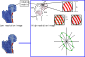
\includegraphics[width=3.5in]{figs/overview.png}
  \caption{Methodology}
  \label{fig:method}
\end{figure}

From the basic implementation, MIL calculation, ellipsoid fitting and region extraction consume approximately {\color{red} 80\%, 15\% and 5 \%} of the overall computing time, respectively. Therefore, we focused on these three algorithms for the optimization. The run time was measured by using time stamp counter (TSC) and the cost analysis of the three algorithm is shown in Table~\ref{tab:cost}.

\mypar{Region extraction}
This algorithm applies a sphere mask on the high resolution image and copies the extraction region to a separate array. A multiplication was performed for each image voxel.

\mypar{Mean Intercept Length (MIL) method}

% todo: add figure of MIL 
The mean intercept length of the vector $v$ can be expressed as:
\begin{equation}
  MIL(v) = \frac{h}{C(v)}
\end{equation}
where $h$ is the summation of the length of all direction vectors and $C(v)$ is the number of intercepts of the vector $v$.
The algorithm includes an addition and a comparison. 
{\color{red}Todo: e.g. explaining about strides}

% todo: algorithm for ellipsoid fitting
\mypar{Ellipsoid fitting}  
{\color{red}Todo}

\begin{table}
  \caption{Cost analysis}
  \label{tab:cost}
  \begin{tabular}{l c c c}
    \toprule
     & flops & read/write & Operational intensity\\
     &   & [doubles] & [flops/double]\\
    \midrule
    Region extractions & $n^{3}$ & $3n^{3}$ & 1/3\\
    MIL \\
    Ellipsoid fitting\\
    \bottomrule
  \end{tabular}
\end{table}


\section{Methods}\label{sec:yourmethod}

% todo: 
% - basic implementation, quantify the perentage of each algorithm takes.
% - testing machine


\mypar{Region extraction} Loop unrolling


\mypar{MIL} Loop unrolling and scalar replacement, blocking, SIMD blocking.

\mypar{Ellipsoid fitting} moving loop invariant code, SIMD


\section{Experimental Results}\label{sec:exp}

The experimental results are presenting here according to the algorithms.

\mypar{Region extraction} \textit{Experimental setup} The tests were performed on Intel i7 U7600 (Kaby Lake), 2.8 GHz without Turboboost. The L1, L2 and L3 cache size were 32KB, 256KB, and 8MB, respectively. The highest optimization flag was used without vectorization (\texttt{-O3 -fno-vectorize-tree}). The sphere region size were ranged from $n=8^{3}$ to $128^{3}$.

\textit{Results} As seen in Fig.~\ref{res:regions}, the loop unrolling method did not improve the performance for the region extraction algorithms.
\begin{figure}[H]
  \centering
 
  \includegraphics[width=3.5in]{figs/plots/regions/regions_performance_labelled.png}
  \caption{Performance of region extraction}
  \label{res:regions}
\end{figure}


\mypar{MIL calculation} \textit{Experimental setup}

\textit{Results}

\begin{figure}[H]
  \centering
  \includegraphics[width=3.5in]{figs/plots/mil/mil_performance_labelled.png}
  \caption{Performance of MIL}
  \label{res:mil}
\end{figure}


\mypar{Ellipsoid fitting} \textit{Experimental setup}

\textit{Results}
 
\begin{figure}[H]
  \centering \includegraphics[width=3.5in]{figs/plots/ellipsoid/ellipsoid_performance_labelled.png}
  \caption{Performance of ellipsoid}
  \label{res:ellipsoid}
\end{figure}


\mypar{Overall performance}

\section{Conclusions}

The bone anisotropy mapping was integrated and optimized. MIL calculation consumes the large percentage of the overall computation time, followed by ellipsoid fitting and region extraction. 

The performance of region extraction was bounded by the intructions mix when it was in cache and memory bound when in memory. The loop unrolling did not improve the performance and the compiler already optimized the alias checking in the basic implementation.

MIL calculation\\

Ellipsoid fitting\\


\section{Further comments}

Here we provide some further tips.

\mypar{Further general guidelines}

% References should be produced using the bibtex program from suitable
% BiBTeX files (here: bibl_conf). The IEEEbib.bst bibliography
% style file from IEEE produces unsorted bibliography list.
% -------------------------------------------------------------------------
\bibliographystyle{IEEEbib}
\bibliography{bibl_conf}

\end{document}

